
%(BEGIN_QUESTION)
% Copyright 2014, Tony R. Kuphaldt, released under the Creative Commons Attribution License (v 1.0)
% This means you may do almost anything with this work of mine, so long as you give me proper credit

Use these graphs to determine the time it will take for a 51 relay to trip given a 600:5 CT ratio, a fault current of 7500 amps, a time-dial setting of 3, and a pick-up current setting (``tap setting'') of 4.0 amps:

$$\epsfxsize=6in \includegraphics[width=15.5cm]{i03329x01.eps}$$

\underbar{file i03329}
%(END_QUESTION)





%(BEGIN_ANSWER)

A fault current of 7500 amps yields a CT secondary current 120 times less than that (5:600 current reduction ratio), or 62.5 amps.  This CT current is 15.625 times greater than the pickup value of 4.0 amps, so we begin our interpretation of the graph by finding 15.625 on the horizontal axis.  A vertical line is already placed at 15$\times$, so we can follow that line and be very close to the true value.

\vskip 10pt

Seeing the point at which the 15$\times$ vertical line crosses the ``3'' time-dial curve and then looking horizontally to the left where it reads out as time, we see a value slightly larger than 0.6 seconds.

\vskip 10pt

\noindent
{\it The graph shown in the question is sampled from the SEL-551 Relay instruction manual, used with permission from Schweitzer Engineering Laboratories.}

%(END_ANSWER)





%(BEGIN_NOTES)


%INDEX% Protective relay: time-overcurrent (51)

%(END_NOTES)


